\documentclass{standalone}
\usepackage{tikz}
\usetikzlibrary{calc}
\begin{document}

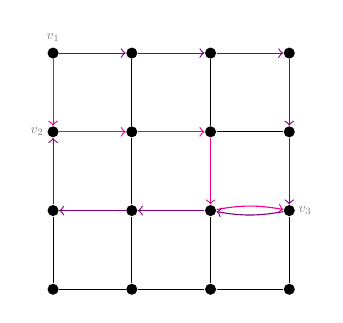
\begin{tikzpicture}[
  every node/.style={circle, fill=black, inner sep=1pt, minimum size=4pt}
]
  \node[label={[gray, scale=0.5]above:$v_1$}] (a) at (0,3) {};
  \node (b) at (1,3) {};
  \node (c) at (2,3) {};
  \node (d) at (3,3) {};
  \node[label={[gray, scale=0.5]left:$v_2$}] (e) at (0,2) {};
  \node (f) at (1,2) {};
  \node (g) at (2,2) {};
  \node (h) at (3,2) {};
  \node (i) at (0,1) {};
  \node (j) at (1,1) {};
  \node (k) at (2,1) {};
  \node (l)[label={[gray, scale=0.5]right:$v_3$}] at (3,1) {};
  \node (m) at (0,0) {};
  \node (n) at (1,0) {};
  \node (o) at (2,0) {};
  \node (p) at (3,0) {};


  \draw (a) edge[->, violet](b);
  \draw (b) edge[->, violet](c);
  \draw (c) edge[->, violet](d);
  \draw (d) edge[->, violet](h);
  \draw (h) edge[->, violet](l);
  
  \draw (k) edge[->, violet](j);
  \draw (j) edge[->, violet](i);
  \draw (i) edge[->, violet](e);

  \draw (a) edge[->, magenta](e);
  \draw (e) edge[->, magenta](f);
  \draw (f) edge[->, magenta](g);
  \draw (g) edge[->, magenta](k);
  \draw[->, magenta] (k) to[bend left=10] (l);
\draw[->, violet] (l) to[bend left=10] (k);

  \draw (b) edge[-](f);
  \draw (c) edge[-](g);
  \draw (g) edge[-](h);
  \draw (f) edge[-](j);
  
  \draw (i) edge[-](m);
  \draw (j) edge[-](n);
  \draw (k) edge[-](o);
  \draw (l) edge[-](p);
  \draw (m) edge[-](n);
  \draw (n) edge[-](o);
  \draw (o) edge[-](p);

\end{tikzpicture}

\end{document}
